%%%%%%%%%%%%%%%%%%%%%%%%%%%%%%%%%%%%%%%%%
% Lachaise Assignment
% LaTeX Template
% Version 1.0 (26/6/2018)
%
% This template originates from:
% http://www.LaTeXTemplates.com
%
% Authors:
% Marion Lachaise & François Févotte
% Vel (vel@LaTeXTemplates.com)
%
% License:
% CC BY-NC-SA 3.0 (http://creativecommons.org/licenses/by-nc-sa/3.0/)
% 
%%%%%%%%%%%%%%%%%%%%%%%%%%%%%%%%%%%%%%%%%

%----------------------------------------------------------------------------------------
%	PACKAGES AND OTHER DOCUMENT CONFIGURATIONS
%----------------------------------------------------------------------------------------

\documentclass{article}

%%%%%%%%%%%%%%%%%%%%%%%%%%%%%%%%%%%%%%%%%
% Lachaise Assignment
% Structure Specification File
% Version 1.0 (26/6/2018)
%
% This template originates from:
% http://www.LaTeXTemplates.com
%
% Authors:
% Marion Lachaise & François Févotte
% Vel (vel@LaTeXTemplates.com)
%
% License:
% CC BY-NC-SA 3.0 (http://creativecommons.org/licenses/by-nc-sa/3.0/)
% 
%%%%%%%%%%%%%%%%%%%%%%%%%%%%%%%%%%%%%%%%%

%----------------------------------------------------------------------------------------
%	PACKAGES AND OTHER DOCUMENT CONFIGURATIONS
%----------------------------------------------------------------------------------------

\usepackage{amsmath,amsfonts,stmaryrd,amssymb} % Math packages
\usepackage[dvipsnames]{xcolor}
\usepackage{enumerate} % Custom item numbers for enumerations
\usepackage{hyperref}
\usepackage[ruled,vlined]{algorithm2e} % Algorithms

\usepackage[framemethod=tikz]{mdframed} % Allows defining custom boxed/framed environments

\usepackage{listings} % Required for insertion of code

\newcommand{\randomcolor}{%
  \definecolor{randomcolor}{RGB}
   {
    \pdfuniformdeviate 256,
    \pdfuniformdeviate 256,
    \pdfuniformdeviate 256
   }%
  \color{randomcolor}%
}

\definecolor{codegreen}{rgb}{0,0.6,0}
\definecolor{codegray}{rgb}{0.5,0.5,0.5}
\definecolor{codepurple}{rgb}{0.58,0,0.82}
\definecolor{backcolour}{rgb}{1,1,1}
\lstdefinestyle{mystyle}{
    backgroundcolor=\color{backcolour},   
    commentstyle=\color{codegreen},
    keywordstyle=\color{magenta},
    numberstyle=\tiny\color{codegray},
    stringstyle=\color{codepurple},
    basicstyle=\ttfamily\footnotesize,
    breakatwhitespace=false,         
    breaklines=true,                 
    captionpos=b,                    
    keepspaces=true,                 
    numbers=left,                    
    numbersep=5pt,                  
    showspaces=false,                
    showstringspaces=false,
    showtabs=false,                  
    tabsize=2
}
\renewcommand{\lstlistingname}{Código}% Listing -> Algorithm
\lstset{style=mystyle}


%\usepackage{listings} % File listings, with syntax highlighting
%\lstset{
%	basicstyle=\ttfamily, % Typeset listings in monospace font
%}

%----------------------------------------------------------------------------------------
%	DOCUMENT MARGINS
%----------------------------------------------------------------------------------------

\usepackage{geometry} % Required for adjusting page dimensions and margins

\geometry{
	paper=a4paper, % Paper size, change to letterpaper for US letter size
	top=2.5cm, % Top margin
	bottom=3cm, % Bottom margin
	left=2.5cm, % Left margin
	right=2.5cm, % Right margin
	headheight=14pt, % Header height
	footskip=1.5cm, % Space from the bottom margin to the baseline of the footer
	headsep=1.2cm, % Space from the top margin to the baseline of the header
	%showframe, % Uncomment to show how the type block is set on the page
}

%----------------------------------------------------------------------------------------
%	FONTS
%----------------------------------------------------------------------------------------

\usepackage[utf8]{inputenc} % Required for inputting international characters
\usepackage[T1]{fontenc} % Output font encoding for international characters

\usepackage{XCharter} % Use the XCharter fonts
\usepackage{pgfplots}
\usepackage{multicol}
%----------------------------------------------------------------------------------------
%	COMMAND LINE ENVIRONMENT
%----------------------------------------------------------------------------------------

% Usage:
% \begin{commandline}
%	\begin{verbatim}
%		$ ls
%		
%		Applications	Desktop	...
%	\end{verbatim}
% \end{commandline}

\mdfdefinestyle{commandline}{
	leftmargin=10pt,
	rightmargin=10pt,
	innerleftmargin=15pt,
	middlelinecolor=black!50!white,
	middlelinewidth=2pt,
	frametitlerule=false,
	backgroundcolor=black!5!white,
	frametitle={Command Line},
	frametitlefont={\normalfont\sffamily\color{white}\hspace{-1em}},
	frametitlebackgroundcolor=black!50!white,
	nobreak,
}

% Define a custom environment for command-line snapshots
\newenvironment{commandline}{
	\medskip
	\begin{mdframed}[style=commandline]
}{
	\end{mdframed}
	\medskip
}

%----------------------------------------------------------------------------------------
%	FILE CONTENTS ENVIRONMENT
%----------------------------------------------------------------------------------------

% Usage:
% \begin{file}[optional filename, defaults to "File"]
%	File contents, for example, with a listings environment
% \end{file}

\mdfdefinestyle{file}{
	innertopmargin=1.6\baselineskip,
	innerbottommargin=0.8\baselineskip,
	topline=false, bottomline=false,
	leftline=false, rightline=false,
	leftmargin=2cm,
	rightmargin=2cm,
	singleextra={%
		\draw[fill=black!10!white](P)++(0,-1.2em)rectangle(P-|O);
		\node[anchor=north west]
		at(P-|O){\ttfamily\mdfilename};
		%
		\def\l{3em}
		\draw(O-|P)++(-\l,0)--++(\l,\l)--(P)--(P-|O)--(O)--cycle;
		\draw(O-|P)++(-\l,0)--++(0,\l)--++(\l,0);
	},
	nobreak,
}

% Define a custom environment for file contents
\newenvironment{file}[1][File]{ % Set the default filename to "File"
	\medskip
	\newcommand{\mdfilename}{#1}
	\begin{mdframed}[style=file]
}{
	\end{mdframed}
	\medskip
}

%----------------------------------------------------------------------------------------
%	NUMBERED QUESTIONS ENVIRONMENT
%----------------------------------------------------------------------------------------

% Usage:
% \begin{question}[optional title]
%	Question contents
% \end{question}

\mdfdefinestyle{question}{
	innertopmargin=1.2\baselineskip,
	innerbottommargin=0.8\baselineskip,
	roundcorner=5pt,
	nobreak,
	singleextra={%
		\draw(P-|O)node[xshift=1em,anchor=west,fill=white,draw,rounded corners=5pt]{%
		Pregunta \theQuestion\questionTitle};
	},
}

\newcounter{Question} % Stores the current question number that gets iterated with each new question

% Define a custom environment for numbered questions
\newenvironment{question}[1][\unskip]{
	\bigskip
	\stepcounter{Question}
	\newcommand{\questionTitle}{~#1}
	\begin{mdframed}[style=question]
}{
	\end{mdframed}
	\medskip
}

%----------------------------------------------------------------------------------------
%	WARNING TEXT ENVIRONMENT
%----------------------------------------------------------------------------------------

% Usage:
% \begin{warn}[optional title, defaults to "Warning:"]
%	Contents
% \end{warn}

\mdfdefinestyle{warning}{
	topline=false, bottomline=false,
	leftline=false, rightline=false,
	nobreak,
	singleextra={%
		\draw(P-|O)++(-0.5em,0)node(tmp1){};
		\draw(P-|O)++(0.5em,0)node(tmp2){};
		\fill[black,rotate around={45:(P-|O)}](tmp1)rectangle(tmp2);
		\node at(P-|O){\color{white}\scriptsize\bf !};
		\draw[very thick](P-|O)++(0,-1em)--(O);%--(O-|P);
	}
}

% Define a custom environment for warning text
\newenvironment{warn}[1][Warning:]{ % Set the default warning to "Warning:"
	\medskip
	\begin{mdframed}[style=warning]
		\noindent{\textbf{#1}}
}{
	\end{mdframed}
}

%----------------------------------------------------------------------------------------
%	INFORMATION ENVIRONMENT
%----------------------------------------------------------------------------------------

% Usage:
% \begin{info}[optional title, defaults to "Info:"]
% 	contents
% 	\end{info}

\mdfdefinestyle{info}{%
	topline=false, bottomline=false,
	leftline=false, rightline=false,
	nobreak,
	singleextra={%
		\fill[black](P-|O)circle[radius=0.4em];
		\node at(P-|O){\color{white}\scriptsize\bf i};
		\draw[very thick](P-|O)++(0,-0.8em)--(O);%--(O-|P);
	}
}

% Define a custom environment for information
\newenvironment{info}[1][Info:]{ % Set the default title to "Info:"
	\medskip
	\begin{mdframed}[style=info]
		\noindent{\textbf{#1}}
}{
	\end{mdframed}
}
 % Include the file specifying the document structure and custom commands

%----------------------------------------------------------------------------------------
%	ASSIGNMENT INFORMATION
%----------------------------------------------------------------------------------------

\title{ITC-ADA-C1-2023: Assignment \#2} % Title of the assignment

\author{Luis Ballado\\ \texttt{luis.ballado@cinvestav.mx}} % Author name and email address

\date{CINVESTAV UNIDAD TAMAULIPAS --- \today} % University, school and/or department name(s) and a date

%----------------------------------------------------------------------------------------

\begin{document}

\maketitle % Print the title

%----------------------------------------------------------------------------------------
%	INTRODUCTION
%----------------------------------------------------------------------------------------

\section{Para los siguientes pares de funciones indique si la primera tiene un orden de crecimiento menor, mayor o igual al de la segunda}

\begin{enumerate}[(a)]
\item $n(n+1)$ y $2000n^{2}$\\
  La primera tiene un orden de crecimiento \textbf{$O(n^2)$} y la segunda también, siendo ambas del mismo orden de crecimiento.
\item $100n^{2}$ y $0,01n^{3}$\\
  La primera tiene un orden de crecimiento \textbf{$O(n^2)$} y la segunda \textbf{$O(n^3)$}, siendo la segunda $O(n^3)$ la función que más rápido crece
\item $\log_{2}n$ y $\ln n$\\
  Considerando a ambas funciones logaritmicas, siendo ambas del mismo orden de crecimiento debido a que forman parte de la misma clase $\Theta(\log n)$
\item $\log_{2}^{2} n$ y $\log_{2}n^{2}$\\\\
  La primera función $\log_{2}^{2} n$ es la función con mayor orden de crecimiento.
\item $2^{n-1}$ y $2^{n}$ \\
  Tienen el mismo orden de crecimiento, forman parte de la misma clase $\Theta(2^{n})$
\item $(n-1)!$ y $n!$ \\
  Tienen el mismo orden de crecimiento, forman parte de la misma clase $\Theta(n!)$
\end{enumerate}

\section{Compare el orden de crecimiento de los siguientes pares de fuciones empleando límites e indique el resultado usando la notación adecuada ($O$,$\Omega$,$\Theta$,etc).}

\begin{enumerate}[(a)]
\item $n!$ y $2^{n}$ \\ Con uso de la formula de stirling donde n! es aproximadamente $\sqrt{2\pi n}(\frac{n}{e})^n$ y al aplicar la regla de l'Hôpital se obtiene:
  \[ \lim_{n\to\infty} \frac{n!}{2^{n}} = \lim_{n\to\infty} \frac{\sqrt{2\pi n} (\frac{n}{e})^n}{2^{n}} = \lim_{n\to\infty} \sqrt{2\pi n}(\frac{n}{2e})^{n} = \infty\], siendo $n!$ la función que más rápido crece $n! \in \Omega(2^{n})$
\item $n^{3}$ y $2^{n}$\\
  \[ \lim_{n\to\infty} \frac{n^{3}}{2^{n}} = \lim_{n\to\infty} \frac{3n^2}{2^{n}\ln (n)} = \infty \], siendo $n^{3}$ la función que más rápido crece $n^{3} \in \Omega (2^{n})$
\end{enumerate}

%----------------------------------------------------------------------------------------
\newpage
\section{Calcule las siguientes sumatorias describiendo en su respuesta las propiedades que emplea en cada paso:}

\begin{enumerate}[(a)]
\item $$ \sum_{i=51}^{100} \left(2i - 1\right)$$ \\
  Haciendo uso de la propiedad 8, separando en intervalos\\
  $$\sum_{i=1}^{100} (2i-1) - \sum_{i=0}^{50}(2i-1)$$\\
  propiedad 7, distribuyendo la sumatoria en los elementos\\
  $$\sum_{i=1}^{100} (2i) + \sum_{i=1}^{100} (-1) - \left(\sum_{i=0}^{50}(2i)+\sum_{i=0}^{50}(-1)\right)$$\\
  propiedad 2\\
  $$\sum_{i=1}^{100}(2i) = \frac{2(100(100+1))}{2} = 10,100$$ \\
  propiedad 1\\
  $$\sum_{i=1}^{100}(-1) = -100 $$\\
  propiedad 2\\
  $$\sum_{i=0}^{50}(2i) = \frac{2(50(50+1))}{2} = 2,550$$\\
  propiedad 1\\
  $$\sum_{i=0}^{50}(-1) = -50 $$\\
  sustituyendo los resultados\\
  10,100 - 100 - 2550 + 50 = 7,500
\item Suponga que $\sum_{i=1}^{5} a_{i}=7$, y $\sum_{i=6}^{12} a_{i}=25$ encuentre el valor de la siguiente sumatoria
  $$\sum_{i=1}^{12} \left(1-a_{i}\right)$$\\
  partiendo de la información brindada, $a_{i}$ en el rango de i=1 hasta 5 toma un valor de 7 y de i=6 hasta 12 toma un valor de 25. Podemos decir que la sumatoria total es 32.\\
  Sustituyendo $$\sum_{i=1}^{12}(a_{i})=32$$ y aplicando la propiedad 1 $$\sum_{i=1}^{12}(1)-32 = 12-32 = -20$$ 
\item Suponga que $ \sum_{i=1}^{5} a_{i}=7$, $\sum_{i=6}^{12} a_{i}=25$ y $\sum_{i=2}^{13} b_{i} = -4$ encuentre el valor de la siguiente sumatoria $$\sum_{i=1}^{12}\left(a_{i}+2b_{i+1}\right)$$\\
  Distribuyendo la sumatoria, aplicando la propiedad 7\\
  $$\sum_{i=1}^{12}(a_{i})+\sum_{i=1}^{12}2b_{i+1}$$\\
  Considerando que $$\sum_{i=2}^{13}b_{i}=-4$$ y que $$\sum_{i=1}^{5}a_{i}=7$$, $$\sum_{i=6}^{12}a_{i}=25$$\\
  $$\sum_{i=1}^{12}a_{i}=32$$ y $$2\sum_{i=1}^{12}(b_{i}) = -8$$\\
  resultando $$32-8=24$$
\item $$ \sum_{k=0}^{99} 2(3^{k})$$\\
  Aplicando la multiplicación\\
  $$\sum_{k=0}^{99} 6^{k}$$\\
  propiedad 4\\
  $$\sum_{k=0}^{99}6^{k}=\frac{6^{k+1}-1}{6-1}=\frac{6^{k+1-1}}{5}$$
\end{enumerate}

\newpage
\section{Considere el algoritmo mostrado y responda las siguientes preguntas:}

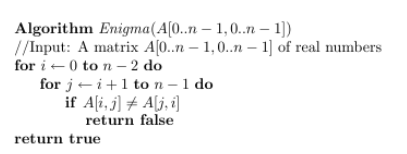
\includegraphics[scale=0.7]{algo.png}

\begin{enumerate}[(a)]
\item ¿Qué calcula el algoritmo?\\
  Dada una matriz, el Algoritmo calcula si ésta es simetrica o no.
\item ¿Cuál es la operación básica?\\
  La operación básica es la comparación de los elementos de la matriz.
\item ¿Cuántas veces se ejecuta la operación básica?
  En el mejor de los casos si dentro de la primera pasada la operación básica regresa que la matriz no es simetrica. En su peor caso deberá recorrer el ciclo anidado for, siendo de complejidad $O(n^2)$, pero el número de comparaciones dependerá del tamaño de la matriz.\\
\item ¿Cuál es la clase de eficiencia a la que petenece este algoritmo?
  $O(n^2)$
\item Sugiera una mejora, o un mejor algoritmo e indique su clase de eficiencia. Si esto no es posible, pruébelo.\\
  No hay un mejor algoritmo, ya que se necesita el doble ciclo for para expolorar la diagonal principal y asegurarnos que no exista diferencia en la comparación para decir que la matriz dada es simetrica.
\end{enumerate}

\section{En un máximo de dos párrafos comente sus conclusiones personales acerca de esta tarea. Podría en ellas tocar algunos de los siguientes puntos: qué aprendí o, qué piensa acerca del uso de estos conceptos matemáticos para analizar algoritmos, qué se le facilitó(dificultó) más al hacer esta tarea, comente un potencial ejemplo de cómo usaría estos conceptos para analizar un algoritmo visto en otro curso, etc.}

Me ayudó a identificar mis deficiencias, para así trabajar en ellas siendo los temas de la notación sigma y el uso adecuado de las notaciones Gran-O,Gran-Omega,Gran-Theta los temas de mayor área de oportunidad que encontré. Los conceptos para la identificación de los ordenes de crecimiento son de gran ayuda, así como en la Ingenieria Cívil responde preguntas del cuanto peso puede soportat una estructura, encontramos en la Ingenieria de Software estas herramientas para poder analizar nuestros algoritmos/códigos y dar respuesta de cuanto tiempo se puede demorar dicho código en base a la cantidad de demanda solicitada. 

\end{document}

